
%% see http://latex-beamer.sourceforge.net/
%% idea contributed by H. Turgut Uyar
%% template based on a template by Till Tantau
%% this template is still evolving - it might differ in future releases!

\documentclass[xcolor={usenames,dvipsnames}]{beamer}
\usepackage{booktabs}
\hypersetup{colorlinks,linkcolor=,urlcolor=}


% THEME
% =========================================================
%\usetheme{Boadilla}
\setbeamertemplate{navigation symbols}{}
\setbeamercolor{normal text}{fg=white,bg=black!90}
\setbeamercolor{structure}{fg=white}
\setbeamercolor{item projected}{use=item,fg=white,bg=item.fg!35}
\setbeamercolor*{palette primary}{use=structure,fg=structure.fg}
\setbeamercolor*{palette secondary}{use=structure,fg=structure.fg!95!black}
\setbeamercolor*{palette tertiary}{use=structure,fg=structure.fg!90!black}
\setbeamercolor*{palette quaternary}{use=structure,fg=structure.fg!95!black,bg=black!80}
\setbeamercolor*{framesubtitle}{fg=white}
\setbeamercolor*{block title}{parent=structure,bg=black!60}
\setbeamercolor*{block body}{fg=black,bg=black!10}
\setbeamercolor*{block title alerted}{parent=alerted text,bg=black!15}
\setbeamercolor*{block title example}{parent=example text,bg=black!15}

\setbeamercolor{mybox}{fg=white,bg=GreenYellow}
%\useinnertheme[shadow]{rounded}
% =========================================================

% DEFINE COLORS
% =========================================================
\definecolor{darkred}{RGB}{223,63,00}
\definecolor{brightred}{RGB}{255,127,00}
% =========================================================

% Templates
% =========================================================
%\setbeamertemplate{itemize subitem}[triangle]
% =========================================================

% SET COLORS
% =========================================================
\setbeamercolor{normal text}{fg=white,bg=black!90}
\setbeamercolor{structure}{fg=white}
\setbeamercolor{item projected}{use=item,fg=white,bg=item.fg!35}
\setbeamercolor*{palette primary}{use=structure,fg=structure.fg}
\setbeamercolor*{palette secondary}{use=structure,fg=structure.fg!95!black}
\setbeamercolor*{palette tertiary}{use=structure,fg=structure.fg!90!black}
\setbeamercolor*{palette quaternary}{use=structure,fg=structure.fg!95!black,bg=black!80}
\setbeamercolor*{framesubtitle}{fg=white}
\setbeamercolor*{block title}{parent=structure,bg=black!60}
\setbeamercolor*{block body}{fg=black,bg=black!10}
\setbeamercolor*{block title alerted}{parent=alerted text,bg=black!15}
\setbeamercolor*{block title example}{parent=example text,bg=black!15}
% =========================================================


% FONTS
% =========================================================
\setbeamerfont{alerted text}{series=\bfseries}
% =========================================================


% PACKAGES
% =========================================================
\usepackage[english]{babel}
\usepackage[utf8]{inputenc}
\usepackage{DejaVuSansMono}
\usepackage[T1]{fontenc}
\usepackage{tikz}
% =========================================================

% METADATA
% =========================================================
\title[CFPS WS~22]{CFPS --- WS 2022}

\subtitle{Seminar}

\author[M. Tschirschnitz]
{
	Maximilian von Tschirschnitz
}

\institute[Chair I20, TUM]
{
	Lehrstuhl f\"ur Sicherheit in der Informatik / I20 \\
	Prof.\ Dr.\ Claudia Eckert\\
	Technische Universität München
}

\date{Oct 25, 2022}
% =========================================================



% If you have a file called "university-logo-filename.xxx", where xxx
% is a graphic format that can be processed by latex or pdflatex,
% resp., then you can add a logo as follows:

% \pgfdeclareimage[height=0.5cm]{university-logo}{university-logo-filename}
% \logo{\pgfuseimage{university-logo}}



% Delete this, if you do not want the table of contents to pop up at
% the beginning of each subsection:
%\AtBeginSubsection[]
%{
%\begin{frame}<beamer>
%\frametitle{Outline}
%\tableofcontents[currentsection,currentsubsection]
%\end{frame}
%}

% If you wish to uncover everything in a step-wise fashion, uncomment
% the following command:

%\beamerdefaultoverlayspecification{<+->}

\begin{document}

\begin{frame}
\titlepage
\end{frame}

%\begin{frame}
%\frametitle{Overview}
%\tableofcontents
%% You might wish to add the option [pausesections]
%\end{frame}

\begin{frame}
	\frametitle{Paper Writing}

	\alert{Disclaimer:} Other disciplines (than Computer Science) and even other sub-disciplines in CS may have their own style on how to structure research papers!

	\vspace{1em}
	The following is \alert{one possible} way out of many. Every paper has it's own dynamics and different things make sense.
\end{frame}

\begin{frame}[plain,c]
	\begin{center}
		\Huge Classical Research Papers
	\end{center}
\end{frame}

\begin{frame}
	\frametitle{Structure}

	\begin{columns}
		\begin{column}{0.5\linewidth}
			\begin{enumerate}
				\item Abstract
				\item Introduction
				\item Related Work
				\item Background
				\item \emph{Your stuff}
				\item Evaluation
				\item Discussion
				\item Conclusion / Future Work
			\end{enumerate}
		\end{column}
	\end{columns}
\end{frame}

\begin{frame}
	\frametitle{Alternative Structure}

	\begin{columns}
		\begin{column}{0.5\textwidth}
			\begin{enumerate}
				\item Abstract
				\item Introduction
				\item Background
				\item \emph{Your stuff}
				\item Evaluation
				\item Discussion
				\item Related Work
				\item Conclusion / Future Work
			\end{enumerate}
		\end{column}
		\begin{column}{0.5\textwidth}
			\alert{Sometimes the reader needs knowledge about your work before they can understand the related work part.}
		\end{column}
	\end{columns}
\end{frame}

\begin{frame}
	\frametitle{General Stuff}

	\begin{itemize}
		\item Prefer \emph{direct speech} over indirect speech.
		\item You may use the scientific \emph{We} when you write
		\item Do not use shortened forms like: \alert{Don't}, \alert{We'll} or \alert{Kinda}
		\item Decide if you want to write \emph{American} or \emph{British English}. Be consistent!
	\end{itemize}
\end{frame}

\begin{frame}
	\frametitle{General Stuff II}

	\begin{itemize}
		\item English sentences commonly do not have a deeply nested sentence structure!

		\item You may want to structure your paragraphs in: Statement, Explanation, Example style.

		\item Reference \alert{all} figures, tables in your text!

		\item Try to be \alert{precise} in your formulation!
			\begin{itemize}
				\item this doesn't necessarily mean it has to be complicated!
			\end{itemize}
	\end{itemize}
\end{frame}

\begin{frame}
	\frametitle{Abstract}

	\begin{itemize}
		\item Extent: \alert{170 - 250 words} (my impression from ACM CCS 2019)
		\item Informal! Do not cite!
	\end{itemize}

	Structure
	\begin{itemize}
		\item Motivation - Why do we care?
		\item Problem Statement - What problem are we trying to solve?
		\item Approach - How did we go about solving?
		\item Result - What is the answer to the problem?
		\item Conclusions - What are the implications?
	\end{itemize}

	{\footnotesize See also \url{https://users.ece.cmu.edu/~koopman/essays/abstract.html}}
\end{frame}

\begin{frame}
	\frametitle{Introduction}

	\begin{columns}
		\begin{column}{0.5\textwidth}
			\begin{itemize}
				\item Motivation for problem
				\item Extent: Usually \alert{one} page!
				\item High-Level Overview of the problem and the structure of the paper.
				\item Clearly state your \alert{contributions} in the end.
			\end{itemize}
		\end{column}
		\begin{column}{0.5\textwidth}
			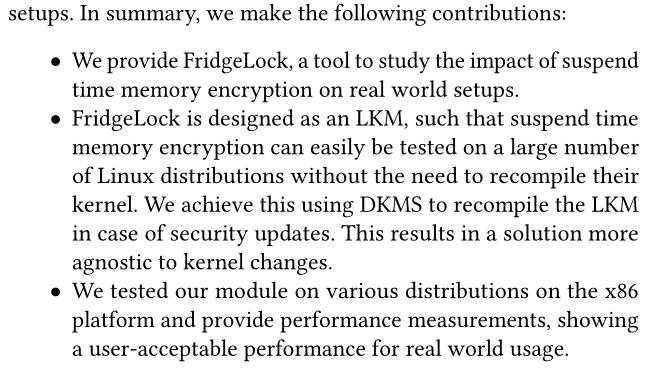
\includegraphics[width=\linewidth]{contributions.png}
		\end{column}
	\end{columns}
\end{frame}

\begin{frame}
	\frametitle{Related Work}

	\begin{itemize}
		\item Makes the reviewer or editors task easier: What is so novel about your work?
		\item Therefore you state in this section what has already been done on this topic.
		\item Give a wide overview only shortly introducing other approaches.
	\end{itemize}
\end{frame}

\begin{frame}
	\frametitle{Background}

	Explain the foundations of the problem to the reader.
\end{frame}

\begin{frame}
	\frametitle{\emph{Your stuff}}
	
	This is your main part! ;)\\[2em]
	You describe here your...
	\begin{itemize}
		\item idea
		\item methodology
		\item implementation (if applicable)
	\end{itemize}
\end{frame}

\begin{frame}
	\frametitle{Evaluation}

	\begin{itemize}
		\item How did you \alert{test} your work?
			\begin{itemize}
				\item How have you made sure it works in all cases?
			\end{itemize}
		\item How does it perform...
			\begin{itemize}
				\item performance-wise?
				\item in comparison to other approaches?
			\end{itemize}
	\end{itemize}
\end{frame}

\begin{frame}
	\frametitle{Discussion}

	\begin{itemize}
		\item Defend your work against anything the reader might not like...
			\begin{itemize}
				\item How much impact has your work?
				\item What does the evaluation suggest?
				\item What are the limitations?
			\end{itemize}
	\end{itemize}
\end{frame}

\begin{frame}
	\frametitle{Conclusion}

	\begin{itemize}
		\item Take a step back from your deep technical writing and summarize one last time what the reader has just learned.
		\item You may want to incorporate the next steps you are planning to do (Future Work).
	\end{itemize}
\end{frame}

\begin{frame}
	\frametitle{SoK: Structure}

	Similar as for Classic Research Papers, but \emph{Related Work} is skipped and \emph{Your Stuff} is ...
	\begin{itemize}
		\item \alert{systematization} of the research field
			\begin{itemize}
				\item adds structure
				\item identifies questions and problem statements
			\end{itemize}
		\item \alert{categorization} of others work
			\begin{itemize}
				\item outlines the basic idea, limitations and implications of every surveyed paper
				\item compares surveyed papers
			\end{itemize}
	\end{itemize}
\end{frame}

\begin{frame}
	\frametitle{SoK: Overview Table Example}

	\begin{center}
		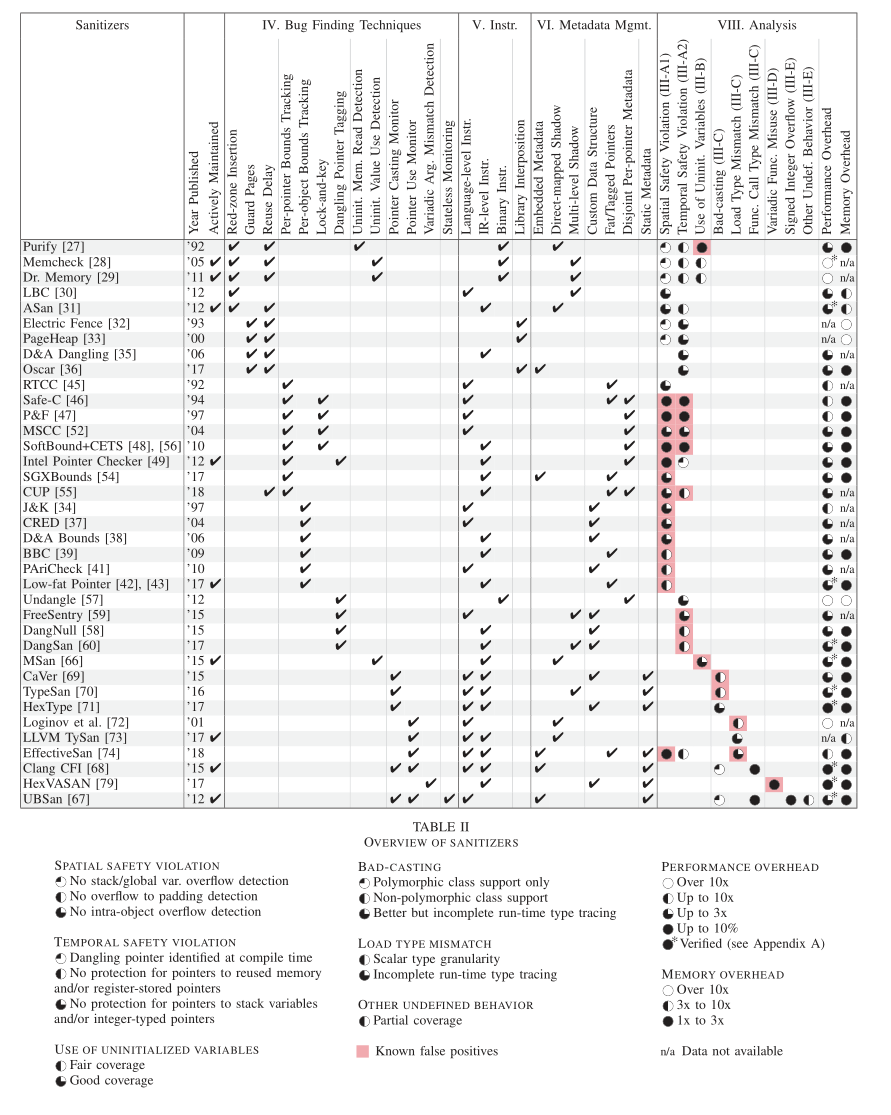
\includegraphics[scale=0.25]{sok-table.png}
	\end{center}
\end{frame}

%\begin{frame}
%	\frametitle{SoK: Overview Table Example II}
%
%	\begin{center}
%		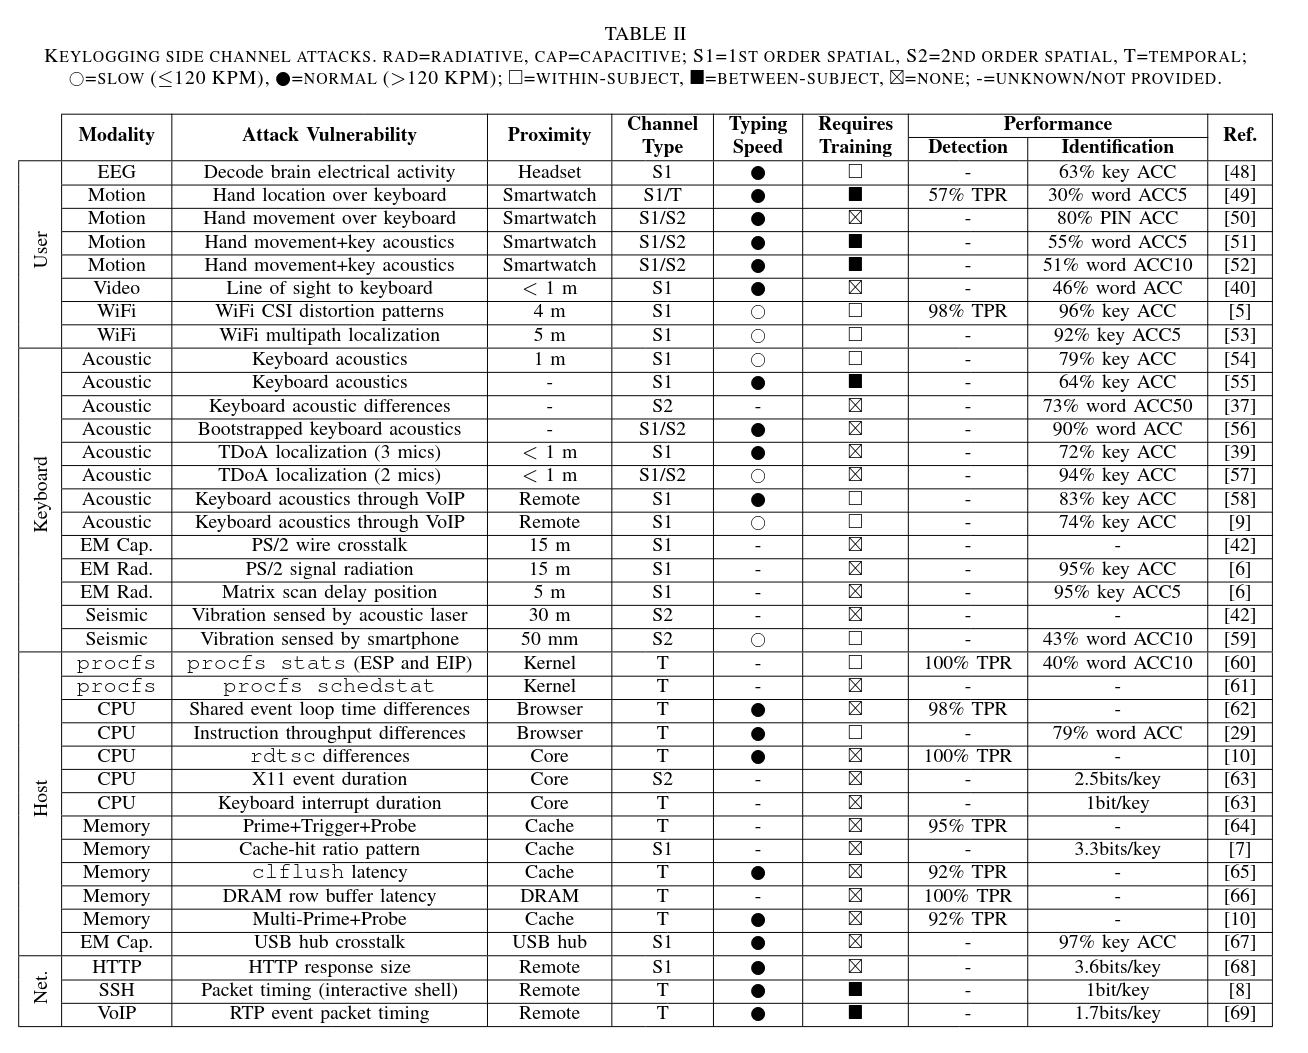
\includegraphics[width=\textwidth]{sok-table2.png}
%	\end{center}
%\end{frame}

\begin{frame}
	\frametitle{Important}
	\alert{Every part of your paper has to have a golden thread easily recognizable.}\newline\newline
	\alert{Making fancy complicated sounding papers is easy, making easy to understand text is the skill!}\newline

	\textbf{What we read on this topic:}\newline
	\emph{Steven Pinker's} - The Sense of Style \url{https://www.goodreads.com/book/show/20821371-the-sense-of-style}\newline\newline
	\emph{Constance Hale's} - Sin and Syntax \url{https://www.goodreads.com/book/show/310014.Sin_and_Syntax}\newline\newline
	\emph{William Zinssner} - On writing Well \url{https://www.goodreads.com/book/show/53343.On_Writing_Well}
\end{frame}

\begin{frame}
	\frametitle{Questions?}
\end{frame}
\end{document}

